\documentclass{article} % For LaTeX2e
\usepackage{nips13submit_e,times}
\usepackage{hyperref}
\usepackage{url}
\usepackage{float}
\usepackage{xcolor}
\usepackage{amsmath}
\usepackage{amssymb}
\usepackage{graphicx}
\usepackage{subcaption}
\newcommand\ytl[2]{
\parbox[b]{8em}{\hfill{\color{black}\bfseries\sffamily #1}~$\cdots\cdots$~}\makebox[0pt][c]{$\bullet$}\vrule\quad \parbox[c]{9cm}{\vspace{7pt}\color{black!40!black!80}\raggedright\sffamily #2.\\[7pt]}\\[-3pt]}

%\documentstyle[nips13submit_09,times,art10]{article} % For LaTeX 2.09


\title{Image Colorization using CycleGAN}

\author{
Zahil Shanis \\
CSE, University at Buffalo\\
Person Number: 50291495\\
\texttt{zahilsha@buffalo.edu} \\
\And
Yash Narendra Saraf \\
CSE, University at Buffalo\\
Person Number: 50290453\\
\texttt{ysaraf@buffalo.edu} \\
\And
Sai Varun Alapati \\
CSE, University at Buffalo\\
Person Number:50290571 \\
\texttt{saivarun@buffalo.edu} \\
}

% The \author macro works with any number of authors. There are two commands
% used to separate the names and addresses of multiple authors: \And and \AND.
%
% Using \And between authors leaves it to \LaTeX{} to determine where to break
% the lines. Using \AND forces a linebreak at that point. So, if \LaTeX{}
% puts 3 of 4 authors names on the first line, and the last on the second
% line, try using \AND instead of \And before the third author name.

\newcommand{\fix}{\marginpar{FIX}}
\newcommand{\new}{\marginpar{NEW}}

\nipsfinalcopy % Uncomment for camera-ready version

\begin{document}


\maketitle

\begin{abstract}

Image-to-image translation is a class of computer vision problem where the goal is to learn the mapping between an input and output image domain using training sets of images from both domains. Artificially coloring grayscale images using deep learning is an application of image to image translation which has produced several compelling results recently in the literature. CycleGAN\cite{cyclegan}, a GAN based unsupervised image-to-image translation architecture proposed by Zhu et. al in 2017, have been used for a wide variety of geometric and color transformations. In this project we investigate a promising method for unsupervised image colorization task using CycleGAN\cite{cyclegan} architecture using Oxford Flower\cite{flower} dataset. We also explore 2 network modifications to the original CycleGAN architecture for image colorization - 1) Using capsule networks\cite{capsnet} as discriminators for the adversarial networks, 2) Implementing a stochastic version of CycleGAN architecture to generate more than one color images for a single grayscale image. We also train a pix2pix\cite{pix2pix} architecture for image colorization to compare the performance of unsupervised image colorization against supervised image colorization.

\end{abstract}

\section{Introduction}
Automated colorization of black and white images has
been subject to much research within the computer vision
and machine learning communities. This problem is not only interesting from an aesthetics perspective, but also has several important applications, including video restoration and image enhancement for better interpretability. Automatic colorization also allows us to appreciate old photographs for which we don't have paired data for training. A machine driven colorization algorithm also helps us to visualize images with different styles, textures and coloring patterns.


In recent years, CNNs have emerged as the de facto standard for solving image classification problems, achieving
error rates lower than 4\% in the ImageNet challenge \cite{imagenet}. Success of deep learning based techniques is primarily attributed to CNN's ability to learn
and discern colors, patterns, and shapes within images and
associate them with object classes. We believe that these
characteristics naturally lend themselves well to colorizing
images since object classes, patterns, and shapes generally
correlate with color choice. With the invention of Generative Adversarial Networks \cite{gan} in 2014, GAN based architectures became prominent of image transformation and styling. These networks are capable of performing style, content and texture transformation to images without having to explicitly train on paired images.

Generally in supervised learning, the algorithm needs to be trained on paired images to teach the system to perform the required task. But it's not always feasible to have a paired sets of training data for all the problems we are trying to solve. Image colorization is one such problem. It's hard to find paired set of images for image colorization if we are specifically dealing with old photos. So, in order to  take this issue also into account, we decided to explore an unpaired image-to-image translation network for image colorization. 

In this project, we try out three different approaches for image colorization task: The first approach involves the use of a cycleGAN architecture to address image colorization as a image-to-image translation problem. Second, we explore the use of capsule networks\cite{capsnet} as discriminators for the cycleGAN architecture to perform image colorization. We also implement a stochastic version of of our GAN architecture to generate multiple color images for a single image. To benchmark the performance of our unpaired image-to-image translation framework, we also train a conditionalGAN architecture which perform image colorization in a supervised manner.

\section{Related work}

Image Colorization is a thoroughly studied problem even before the use of deep learning based techniques. Image colorization was initially done using two main methods i.e. interactive colorization methods, and automatic colorization methods\cite{interactive}. The interactive methods required the user to mark color to different surfaces which are then smoothly propagated across the entire image based on an optimization framework. Many earlier automatic colorization techniques focused on using image processing techniques like Gabor transforms and SIFT keypoint detection \cite{gabor}. 

In 2016  Ryan Dahl’s \cite{ryan} CNN based architecture for automatically colorizing images used a network that integrated ImageNet-trained layers from VGG16\cite{vgg} with an autoencoder like system using residual connections \cite{resnet}. In terms of results, Dahl’s system performed extremely well in realistically colorizing foliage, skies, and skin. Here Dahl formulated image colorization as a regression problem where the objective function was to minimise the a sum of Euclidean distances between each pixel’s blurred color channel values in the target image and predicted image. The regression methods result in inconsistencies if multiple colored copies of same object are present in the dataset as the network would try to average those colors out resulting in a subdued mixture of possible colors. 

In 2016, Richard et al. \cite{richard} proposed a fully automatic approach by posing it as a classification task and use class-rebalancing at training time to increase the diversity of colors in the result. With the advent of Deep Learning, several CNN based architectures were proposed for image colorization. Deep Colorization \cite{deepcolor} of Cheng, Yang, and Sheng (2016) describes a neural network for colorization which input a grayscale image and output a color image in YUV color space. This paper also formulates colorization as a regression problem, with the loss function as a least squares minimization between the predicted and ground-truth color pixel values.

Image-to-image translation\cite{pix2pix} has gained considerable attention due to the recent impressive progress based on generative adversarial networks (GANs).  Generative Adversarial Networks \cite{gan} proposed by Ian Good fellow in 2014 is composed of two smaller networks called the generator and discriminator. 

Several papers have been published which uses GAN architecture for various image transformation tasks including image-to-image translation. Image-to-Image Translation with Conditional Adversarial Networks(pix2pix) of Isola et al.\cite{pix2pix} introduces conditional adversarial networks as a general-purpose solution to image-to-image translation problems like reconstructing objects from edge maps, style transfer, etc. 

Even though pix2pix is capable of generating excellent translations, it requires paired input data for training. This could be infeasible for the cases where we don't have one-to-one matches between the two image profiles (eg: image colorization). CycleGAN \cite{cyclegan} proposed by Zhu et. al overcomes this issue.

The key idea behind CycleGANs\cite{cyclegan} is that they can build upon the power of the pix2pix\cite{pix2pix} architecture, but allow you to point the model at two discrete, unpaired collections of images. CycleGAN framework have been applied for several different image-to-image translation problems, including artists’ styles and photos, apples and oranges, zebras and horses, winter and summer, and maps and aerial photographs and have achieved excellent results\cite{cyclegan_site}. 

In this paper, we develop an unpaired image-to-image translation algorithm which translates grayscale images to color image domain. We use CycleGAN as your base network for image translation and propose various modifications  to the network architecture to generate realistic color images from grayscale counterparts.

\section{Methods}
We use CycleGAN as our backbone network for image colorization. As described earlier, the power of CycleGAN lies in being able to learn such transformations without one-to-one mapping between training data in source and target domains. The need for a paired image in the target domain is eliminated by making a two-step transformation of source domain image - first by trying to map it to target domain and then back to the original source domain. Mapping of image to target domain is done using a generator network and the generated image is translated back to the source domain using another generator network. The quality of the generated images are improved by pitching the generators against a pair of discriminators. A schematic diagram of cycleGAN network is presented in \ref{fig:base}.
\begin{figure}[!htb]
\centering
\begin{subfigure}{.3\textwidth}
  \centering
  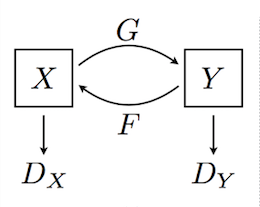
\includegraphics[width=1\linewidth]{cyclegan.png}
  \caption{Basic Architecture of CycleGAN}
  \label{fig:base}
\end{subfigure}%
\begin{subfigure}{.6\textwidth}
  \centering
  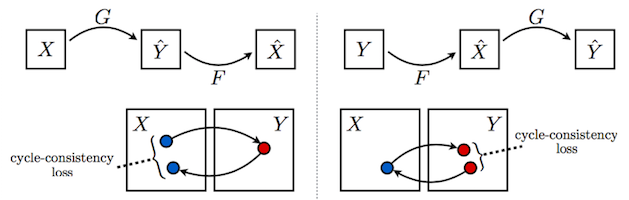
\includegraphics[width=1\linewidth]{cycle_consistency.png}
  \caption{CycleGAN Cycle Consistency Loss}
  \label{fig:consistency}
\end{subfigure}
\caption{CycleGAN Architecture}
\label{fig:cyclegan}
\end{figure}
\subsection{Network Architecture}
CycleGAN is a Generative Adversarial Network (GAN) that uses two generators and two discriminators. We call one generator G, and have it convert images from the X domain to the Y domain. The other generator is called F, and converts images from Y to X. Here, we use X as the grayscale domain and Y as the color domain.
    $$G : X \rightarrow Y$$
    $$F : Y \rightarrow X$$
Additionally, each generator has a corresponding discriminator, which attempts to tell apart its synthesized images from real ones.\newline \newline
$D_x : \text{Distinguishes real grayscale images from the fake grayscale image generated by } F.$ \newline
$D_y : \text{Distinguishes real color images from the fake color image generated by } G.$ 
\newline
\paragraph{Generator Network}: We use the default CycleGAN generator architecture for image colorization. Each CycleGAN generator has three sections: an encoder, a transformer, and a decoder. The input image is fed directly into the encoder, which shrinks the representation size while increasing the number of channels. The encoder is composed of three convolution layers. The resulting activation is then passed to the transformer, a series of six residual blocks. It is then expanded again by the decoder, which uses two transpose convolutions to enlarge the representation size, and one output layer to produce the final image in RGB. Each layer in the generator network is followed by an instance normalization and ReLU layer. 
\paragraph{Discriminator Network}: We use PatchGANs as discriminators. PatchGANS are fully convolutional neural networks that look at a “patch” of the input image, and output the probability of the patch being “real”. This is both more computationally efficient than trying to look at the entire input image, and is also more effective-it allows the discriminator to focus on more surface-level features, like texture, which is often the sort of thing being changed in an image translation task. PatchGAN was first proposed by Isola et al in \cite{pix2pix}.

\subsection{Loss Functions}
The real power of CycleGAN architecture lies in the loss function used by it. In addition to the adversarial loss used by adversarial networks\cite{gan}, CycleGAN also uses a cycle-consistency loss.

\paragraph{Adversarial Loss}: Adversarial losses are applied to both mapping functions. For the mapping function, $G : X \rightarrow Y$ and its discriminator $D_Y$, objective loss can be expressed as:\\
\begin{equation}
    \mathcal{L}_{GAN}(G,D_X,X,Y) = \mathbb{E}_{y\sim p_{data}(y)}\left[\log D_Y(y)\right] + \mathbb{E}_{y\sim p_{data}(y)}\left[\log (1-D_Y(G(x)))\right]
\end{equation}
\newline
where $G$ tries to generate images $G(x)$ that look similar to images from domain $Y$, while $D_Y$ aims to distinguish between translated samples $G(x)$ and real samples $y$. A similar adversarial loss is used for the mapping function $F : Y \rightarrow X$ and its discriminator $D_X$ as well.
\paragraph{Cycle Consistency Loss}: Adversarial loss alone is not sufficient to produce good color images. It ensures that the generated color image belongs to the color image domain, but does not enforce that the input and output are recognizably the same. A cycle consistency loss is used to address this issue. It relies on the expectation that if you convert an image to the other domain and back again, by successively feeding it through both generators, you should get back something similar to what you put in. It enforces that $F(G(x)) ≈ x$ and $G(F(y)) ≈ y$.\\
\begin{equation}\label{eq:cycle_const}
    \mathcal{L}_{cyc}(G,F) = \mathbb{E}_{y\sim p_{data}(y)}\left[|| F(G(x)) - x||_1 \right] + \mathbb{E}_{y\sim p_{data}(y)}\left[|| G(F(y)) - y||_1 \right]
\end{equation}
\newline
Total objective function of CycleGAN is the weighted sum of all the losses.
\newline
\begin{equation}
    \mathcal{L}(G,F,D_X, D_Y) = \mathcal{L}_{GAN}(G,D_X,X,Y) + \mathcal{L}_{GAN}(F,D_Y,Y,X) + \lambda\mathcal{L}_{cyc}(G,F)
\end{equation}

\subsection{Stochastic CycleGAN}
Image translation from grayscale to color images is not a one to one mapping problem. For example, a grayscale image of a scenery can have multiple consistent color image mappings for different seasons. While the mapping that CycleGAN learns can be superficially convincing (e.g. it produces a single reasonable color image with a particular style), we would like to learn a mapping that can capture diversity of the output (e.g. produces multiple images corresponding to multiple styles). We modified the generator network to hallucinate multiple color images for a single grayscale image by adding stochasticity to $G$ network. The idea is based on then notion of Conditional Instance Normalization proposed by V Dumoulin et.al in \cite{cond_norm} where a gaussian prior noise is passed to the Instance Normalization layers of $G : X \rightarrow Y$ network.

\subsection{Capsule Discriminators}

In 2017, Sabour et al. in \cite{capsnet} introduced Capsule Networks as an improvement to the Convolutional Neural Networks. The CNNs use Max Pooling layer for feature reduction which is one of the places where necessary information might get lost. This makes the CNNs less sensitive to spatial relationships between objects. To tackle the same problem the capsule networks were introduced which are more robust to changes in poses and spatial relationships between objects. It was introduced to capture the mechanism in which the optic neurons work in the Human visual system. Capsules are locally invariant groups of neurons that learn to recognize visual entities and output activation vectors that represent both the presence of those entities and their properties. The 2017 paper introduces the training algorithm of CapsNets i.e. a Dynamic routing algorithm between capsules in successive layers of network which imitates hierarchical communication of information across neurons in human brains that are responsible for visual perception and understanding. Capsule The original paper also set the new state of the art for MNIST digit classification and segmentation of overlapping digits. 

This idea was furthered by  Jaiswal et al. in \cite{capsuleGan} where they introduced the Capsule Networks integration along with the GANs. GAN architectures are very difficult to train because of the min-max objective function of the two player game and the possibility of mode collapse. So the paper just uses the Capsule Networks as the Discriminators to make the Discriminator capable of learning better which would in turn help the generator to produce better images. 

\begin{figure}[h]
	\begin{center}
		\fbox{ 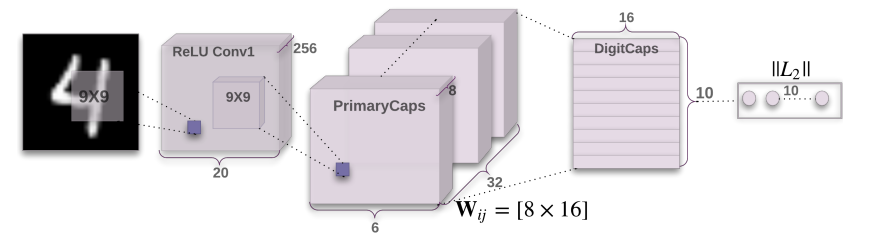
\includegraphics[width=0.8\textwidth]{3.png} }
	\end{center}
	\caption{A simple CapsNet with 3 layers. The length of the activity vector of each capsule in DigitCaps layer indicates presence of an instance of each class and is used to calculate the classification loss.\cite{capsnet} }
\end{figure}

Capsules are locally invariant groups of neurons that learn to recognize the presence of visual entities and encode their properties into vector outputs, with the vector length (limited to being between zero and one using squashing functions) representing the presence of the entity. Sabour et al. in in \cite{capsnet} introduced a routing-by-agreement mechanism for the interaction of capsules within deep neural networks with several capsule-layers, which works by pairwise determination of the passage of information between capsules in successive layers. 


Inspired by the results from CapsuleGAN paper\cite{capsuleGan}, we modified the CycleGAN architecture to use Capsule Networks for discriminator. The discriminator uses three layers of digit capsules which are used to learn complex features from primary capsules. The output is produced using the sigmoid activation for the classification problem as 0 or 1. The loss function used is Binary Cross-entropy to train the discriminator. To reduce the parameters in the Capsule Network architecture the images are scaled down to 32x32 before feeding them to the discriminator. 

\subsection{Conditional GAN}

We also train a ConditionalGAN(pix2pix)\cite{pix2pix} network for image colorization in order to compare unsupervised image-to-image translation with supervised translation. Conditional GANs are trained in a supervised fashion tolearn a mapping from observed image X and random noise vector Z, to Y,  $G :(x,z) \rightarrow Y$. The generator G is trained to produce outputs that cannot be distinguished from “real” images by an adversarialy trained discriminator, D, which is trained to do as well as possible at detecting the generator’s “fakes”. This training procedure is represented in Figure \ref{fig:pix2pix}.

\begin{figure}[!htb]
	\begin{center}
		\fbox{ 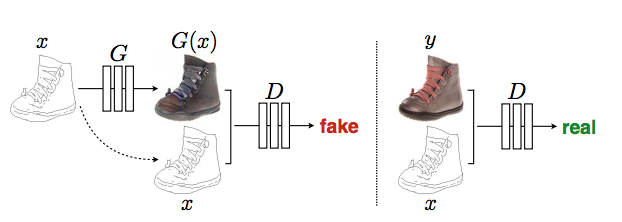
\includegraphics[width=0.8\textwidth]{conditional_gan.png} }
	\end{center}
	\caption{High level overview of Conditional GAN.}
	\label{fig:pix2pix}
\end{figure}

\paragraph{Objective function  :}
ConditionalGAN mixes the GAN objective presented in Eq. 1 with a more traditional supervised loss such as $L_1$ or $L_2$ distance loss. The discriminator’s job remains unchanged, but the generator is tasked to not only fool the discriminator but also to be near the ground truth output at a pixel level. $L_1$ distance is preferred over $L_2$ since $L_2$ encourages blurring.
\begin{equation}
    \mathcal{L}_{L1}(G) = \mathbb{E}_{ x,y,z}\left[||y - G(x,y)||_{1}\right]
\end{equation}

Total objective function of Conditional GAN is the weighted sum of all the losses.
\begin{equation}
    G^* = \mathcal{L}_{cGAN}(G,D) + \lambda\mathcal{L}_{L1}(G)
\end{equation}

\section{Experiments}
\subsection{Image Colorization with CycleGAN}
We used default cycleGAN architecture with minimal changes for image colorization. A keras implementation of CycleGAN was obtained from the Keras GAN Zoo repository hosted by Erik Linder-Norén \cite{cycleGanImpl}. With gray-scale images as domain A and color images as domain B, we trained the network for 200 epochs using various hyper-parameter setup. Cycle consistency loss was applied as a pixel level to penalize the difference between real and reconstructed images.

We obtained preliminary results by training the model on the full dataset for 10 epochs with a learning rate of 0.0002 using Adam optimizer\cite{adam} with β1 = 0.9 and β2 = 0.999 for both discriminator and generator. Batch size of 1 was used with instance normalisation between generators' convolutional layers. We optimize over the weighted sum of the GAN loss and the pixel loss for different choices of loss and weight ratio $\lambda$. We also tried $L_1$ and $L_2$ norms for the cycle consistency losses. Model with $L_2$ cycle consistency loss performed poorly and often generated monochromatic color images. So we decided to stick with the $L_1$ loss as suggested in the original CycleGAN paper\cite{cyclegan}.

CycleGAN architecture with $L_1$ cycle consistency loss achieved perceptually convincing results. Color mappings of a few of the grayscale images are presented in \ref{fig:cyclegan_results}. It's evident from the results that the model is able to understand the underlying mapping from grayscale domain to color domain in a couple of hundred epochs of training. 

\begin{figure}[!htb]
	\begin{center}
		\fbox{ 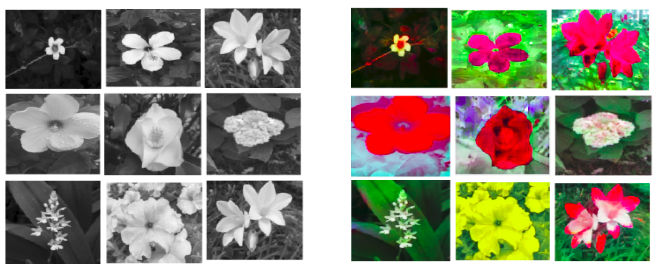
\includegraphics[width=0.9\textwidth]{cyclegan_results.png} }
	\end{center}
	\caption{Grayscale images and corresponding color mappings generated by CycleGAN.}
	\label{fig:cyclegan_results}
\end{figure}

\subsection{Image Colorization with Capsules}

Capsule Networks being powerful at learning hierarchical relationships were used as discriminator network. The architecture used single primary capsule layer along with three softmax digit capsule layers. As the number of parameters required by the capsule Network are quite high the discriminator was modified to take an input of original dimensions i.e. 128x128 and then rescale it to 32x32 before running the classification problem. The last layer is a dense layer with single neuron which uses sigmoid as the function to classify the object. The two loss functions tried out were MSE and binary cross-entropy for the classification. The results turned out to be better with the mean square error. Apart from that the rest of the cycle GAN architecture is similar to the one used above. Some of the results for the capsule networks have been grouped together in the \ref{fig:capsulegan_results} figure-


\begin{figure}[!htb]
	\begin{center}
		\fbox{ 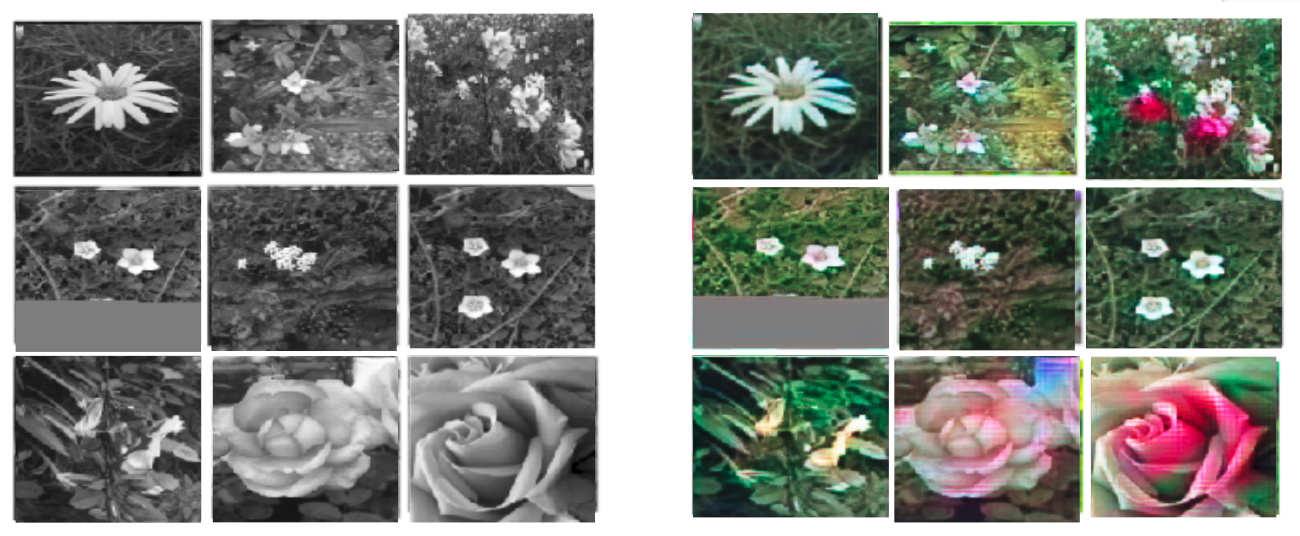
\includegraphics[width=0.9\textwidth]{capsuleGan_results.png} }
	\end{center}
	\caption{Grayscale images and corresponding color mappings generated by CapsuleGAN.}
	\label{fig:capsulegan_results}
\end{figure}

To compare the two approaches we calculated the sum of pixel wise absolute difference between the original colored image and generated image. (Note: the original image used while calculating this was not used while training the model as the pairwise input.). The following is the short summary of comparison between the two approaches discussed above, i.e. PatchGANs AND CapsuleGANs. 

\begin{figure}[!htb]
	\begin{center}
		\fbox{ 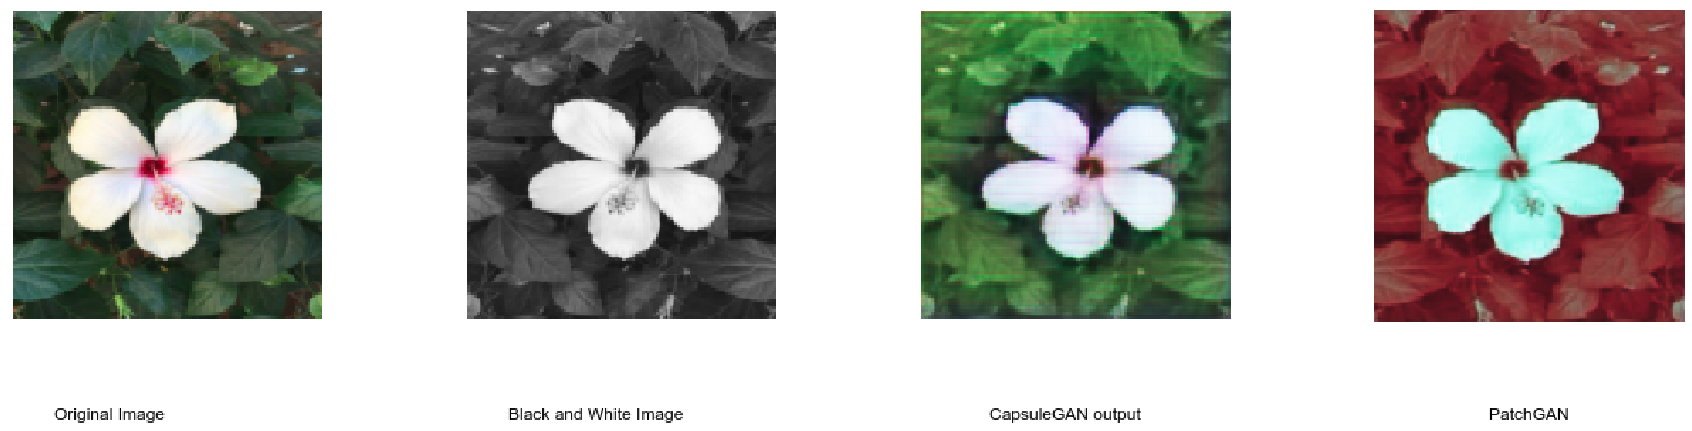
\includegraphics[width=0.9\textwidth]{comparison.png} }
	\end{center}
	\caption{Corresponding images generated by PatchGAN and CapsuleGAN for the same input}
	\label{fig:comparison}
\end{figure}

The mean sum of pixel wise absolute difference for the CapsuleGAN architecture was around 23985.481278488893 whereas it was around 22476.771897710358 for PatchGAN architecture. It was clearly seen that both architectures were performing comparatively same in performance. One major difference which was seen was both architectures were performing better on different images. 

\subsection{Stochastic CycleGAN}
In order to accomplish a one-to-many mapping instead of a one-to-one deterministic mapping for image colorization, we trained the CycleGAN network with stochastic generators. A Gaussian prior noise is passed to the instance normalization layers of $G$ network to introduce stochasticity in the network as suggested in \cite{cond_norm}. The network is trained for 200 epochs without changing any other model parameters.

Contrary to our expectation, stochastic generators produced same images with different gaussian priors. This might be because the cycle-consistency in Eq \ref{eq:cycle_const} encourages the mappings to ignore the latent gaussian noise. Specifically, the unimodality assumption implicit in the reconstruction error from Eq. \ref{eq:cycle_const} forces $G$ and $F$ mappings to be one-to-one.

\subsection{Image Colorization with Conditional GAN}
We used default conditoinalGAN architecture with minimal changes for image colorization. A keras implementation of Conditional GAN was obtained from the Keras GAN Zoo repository hosted by Erik Linder-Norén \cite{conditionalganImpl}. Network is trained in a supervised fashion for 100 epochs using paired training images. Image colorization by conditionalGAN are presented in Figure \ref{fig:conditional_gan_results}.

\begin{figure}[!htb]
	\begin{center}
		\fbox{ 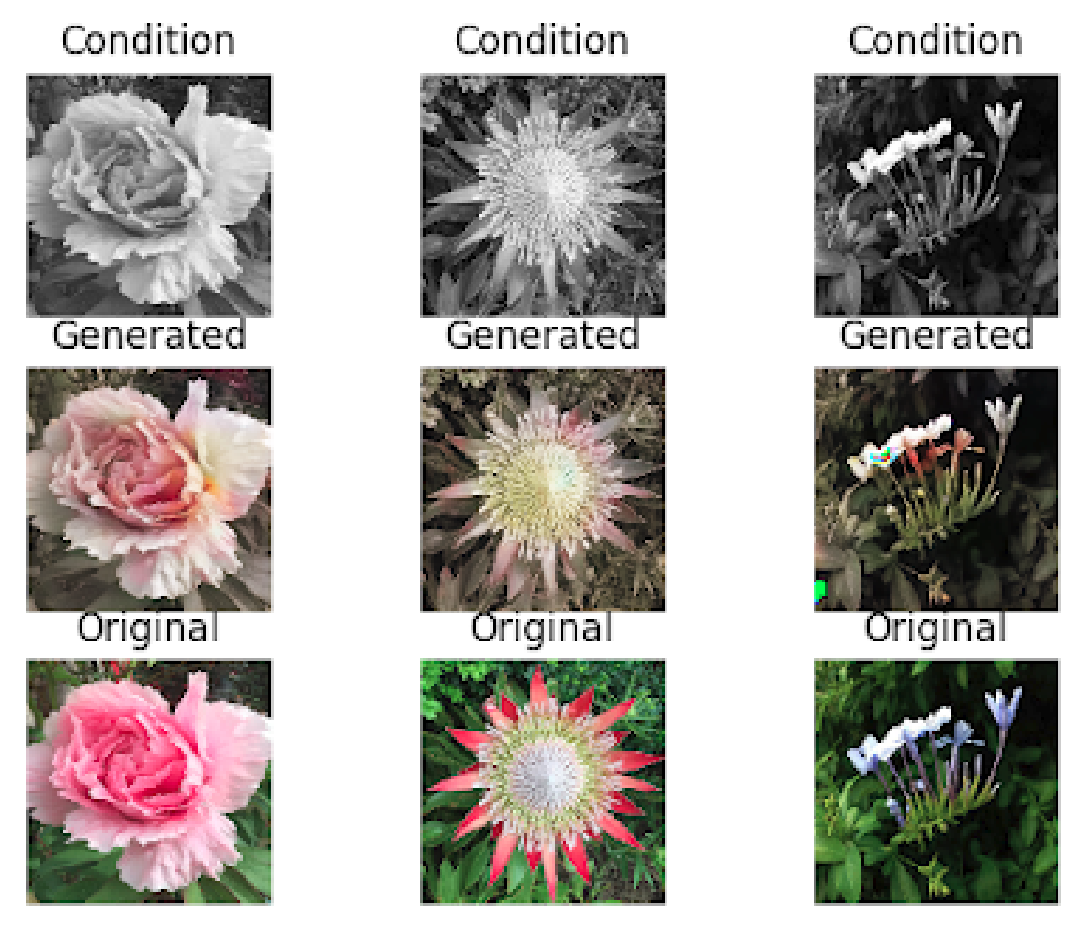
\includegraphics[width=0.7\textwidth]{conditional_gan_result.png} }
	\end{center}
	\caption{Grayscale condition images and corresponding color mappings generated by Conditional GAN.}
	\label{fig:conditional_gan_results}
\end{figure}


\section{Conclusion}
Based on our experiments, it is clear that image-to-image translation networks with cycle consistency are very promising for autocolorization. However, the objective function needs to be carefully designed and tailored to this problem to account for the multimodal nature of the problem. Additionally, we also learned that network cannot be made stochastic by adding Gaussian prior to the generator network.The results we achieved with cycle gan is on a level with the conditional gan which concludes that unsupervised learning is working as good as supervised learning. The CapsuleGAN architecture seems promising as it provided comparable results to the PatchGAN architecture. As caspule networks are able to handle spatial relationships between objects far better than traditional CNNs it would provide a strong foundation for GANs if the model is tuned appropriately. As future improvements a combination of the two can be designed i.e. a capsuleGAN Architecture with Patch output which would help the model to learn the features better. Also the problem can be designed as a semi supervised problem where we use the cycle consistency loss along with the conditional loss to train the model. This would make sure the mapping between the two domains is considered along with the paired images mean square losses. 


\begin{thebibliography}{999}
\bibitem{flower} 
Nilsback, M-E. and Zisserman, A.,
\textit{A Visual Vocabulary for Flower Classification,}. 
Proceedings of the IEEE Conference on Computer Vision and Pattern Recognition, 2006

\bibitem{places} 
B. Zhou, A. Lapedriza, J. Xiao, A. Torralba, and A. Oliva,
\textit{Learning Deep Features for Scene Recognition using Places Database,}. 
Advances in Neural Information Processing Systems 27 (NIPS), 2014

\bibitem{} 
Alex Krizhevsky,
\textit{Learning Multiple Layers of Features from Tiny Images,}. 
\href{https://www.cs.toronto.edu/~kriz/learning-features-2009-TR.pdf}{https://www.cs.toronto.edu/~kriz/learning-features-2009-TR.pdf},
2009

\bibitem{cyclegan} 
Jun-Yan Zhu, Taesung Park, Phillip Isola, and Alexei A. Efros,
\textit{Unpaired Image-to-Image Translation using Cycle-Consistent Adversarial Networks,} 
International Conference on Computer Vision 2017

\bibitem{vgg} 
Karen Simonyan, Andrew Zisserman,
\textit{Very Deep Convolutional Networks for Large-Scale Image Recognition,} 
arXiv, 1409.1556, 2014

\bibitem{resnet} 
Kaiming He, Xiangyu Zhang, Shaoqing Ren, Jian Sun,
\textit{Deep Residual Learning for Image Recognition,} 
arXiv, 1512.03385, 2015

\bibitem{interactive} 
V. Konushin, and V. Vezhnevets. 
\textit{Interactive Image Colorization and Recoloring based on Coupled Map Lattices,}. 
2006 .

\bibitem{gabor} 
Raj Kumar Gupta, Alex Yong-Sang Chia, Deepu Rajan1 Ee Sin Ng, and Huang Zhiyong,
\textit{Image Colorization Using Similar Images,}. 
MM '12 Proceedings of the 20th ACM international conference on Multimedia
Pages 369-378 .

\bibitem{ryan} 
Ryan Dahl,
\textit{Automatic Colorization,}. 
\href{https://tinyclouds.org/colorize/}{https://tinyclouds.org/colorize/},
January 2016.

\bibitem{} 
Medium Blog: Lee Cohn,
\textit{Artificial Colorization of Grayscale Satellite Imagery via GANs: Part 1,}. 
\href{https://medium.com/the-downlinq/artificial-colorization-of-grayscale-satellite-imagery-via-gans-part-1-79c8d137e97b}{https://medium.com/the-downlinq/artificial-colorization-of-grayscale-satellite-imagery-via-gans-part-1-79c8d137e97b},
August 2017

\bibitem{cyclegan_site} 
Github page, Jun-Yan Zhu, Taesung Park, Phillip Isola, and Alexei A. Efros,
 \textit{CycleGAN Applications}. 
\href{https://junyanz.github.io/CycleGAN/}, 2017

\bibitem{capsuleGan} 
Ayush Jaiswal, Wael AbdAlmageed, Yue Wu, Premkumar Natarajan,
\textit{CapsuleGAN: Generative Adversarial Capsule Network,}. 
\href{https://arxiv.org/abs/1802.06167}{https://arxiv.org/abs/1802.06167},
 Brain Driven Computer Vision (BDCV) 2018

\bibitem{capsnet} 
Sara Sabour, Nicholas Frosst, Geoffrey E Hinton,  
\textit{Dynamic Routing Between Capsules,}. 
\href{https://arxiv.org/abs/1710.09829}{https://arxiv.org/abs/1710.09829},
Oct 2017

\bibitem{pix2pix} 
Phillip Isola, Jun-Yan Zhu, Tinghui Zhou, Alexei A. Efros,  
\textit{Image-to-Image Translation with Conditional Adversarial Networks,}. 
\href{https://arxiv.org/pdf/1611.07004.pdf}, arXiv, 1611.07004,
2016

\bibitem{cond_norm} 
Vincent Dumoulin, Jonathon Shlens, Manjunath Kudlur,  
\textit{A learned representation for artistic style,}. 
ICLR, 2017

\bibitem{capsGan} 
Raeid Saqur, Sal Vivona,  
\textit{CapsGAN: Using Dynamic Routing for Generative Adversarial Networks,}. 
\href{https://arxiv.org/abs/1710.09829}{https://arxiv.org/abs/1710.09829},
June 2018

\bibitem{capsImpl} 
Guseyn Gadirov,  
\textit{Capsule GAN - Implementation,}. 
\href{https://github.com/gusgad/capsule-GAN}{https://github.com/gusgad/capsule-GAN},
Feb 2018

\bibitem{deepcolor} 
Zezhou Cheng, Qingxiong Yang, Bin Sheng,
\textit{Deep Colorization,} 
International Conference on Computer Vision, 2015 

\bibitem{richard} 
Zhang R., Isola P., Efros A.A, 
\textit{Colorful Image Colorization,} 
ECCV 2016. Lecture Notes in Computer Science, vol 9907. Springer, Cham

\bibitem{imagenet} 
Olga Russakovsky, Jia Deng, Hao Su, Jonathan Krause and
               Sanjeev Satheesh, Sean Ma, Zhiheng Huang, Andrej Karpathy, Aditya Khosla, Michael S. Bernstein, Alexander C. Berg, Fei{-}Fei Li, 
\textit{ImageNet Large Scale Visual Recognition Challenge,} 
CoRR, abs/1409.0575, 2014

\bibitem{gan} 
Ian Goodfellow, Jean Pouget-Abadie, Mehdi Mirza, Bing Xu, David Warde-Farley, Sherjil Ozair, Aaron Courville, and Yoshua Bengio,
\textit{Generative adversarial nets,} 
Advances in Neural Information Processing Systems pages 2672–2680, 2014.
\bibitem{adam}
Diederick P Kingma, Jimmy Lei Ba,
\textit{Adam: A Method for Stochastic Optimization,} 
ICLR, 2015
\bibitem{cycleGanImpl} 
Erik Linder-Norén,  
\textit{Cycle GAN - Code,}. 
\href{https://github.com/eriklindernoren/Keras-GAN/tree/master/cyclegan},
Feb 2018

\bibitem{conditionalganImpl} 
Erik Linder-Norén,  
\textit{Conditional GAN - Implementation,}. 
\href{https://github.com/eriklindernoren/Keras-GAN/tree/master/pix2pix},
Feb 2018

\end{thebibliography}

\end{document}
